\documentclass[crop,tikz,border=4pt,12pt]{standalone}
\usepackage{amsmath}
\newcommand{\tikzsetnextfilename}[1]{}
\definecolor{profileBlue}{RGB}{156,201,223}
\definecolor{profileStroke}{RGB}{47,58,69}
\definecolor{profileDivider}{RGB}{39,109,100}

% Occupied cells x/y, measured from the bottom left; -1/-1 is empty.
\newcommand{\frontierprofile}[2]{%
  \fill[white] (0,0) rectangle (2,3);
  \foreach \x/\y in {#2}{%
    \ifnum\x>-1\relax
      \fill[profileBlue] (\x,\y) rectangle ++(1,1);
    \fi
  }%
  \draw[profileStroke,step=1,line width=0.5pt] (0,0) grid (2,3);
  \draw[profileDivider,line width=1.2pt] (1,0)--(1,3);
  \node[above,text=profileStroke] at (1,3.15) {$#1$};
}

\begin{document}
\tikzsetnextfilename{transfer-matrix-triomino-profiles}
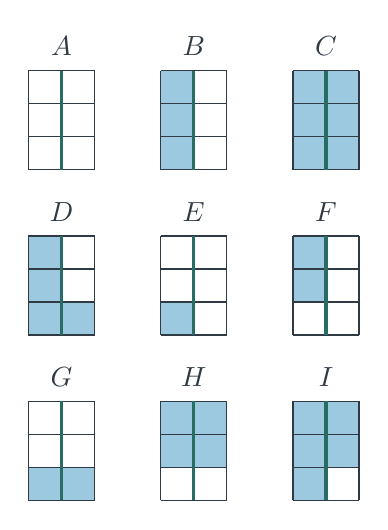
\begin{tikzpicture}[x=0.42cm,y=0.42cm]
  \begin{scope}[shift={(0,10)}]
    \frontierprofile{A}{-1/-1}
  \end{scope}
  \begin{scope}[shift={(4,10)}]
    \frontierprofile{B}{0/0,0/1,0/2}
  \end{scope}
  \begin{scope}[shift={(8,10)}]
    \frontierprofile{C}{0/0,0/1,0/2,1/0,1/1,1/2}
  \end{scope}
  \begin{scope}[shift={(0,5)}]
    \frontierprofile{D}{0/0,0/1,0/2,1/0}
  \end{scope}
  \begin{scope}[shift={(4,5)}]
    \frontierprofile{E}{0/0}
  \end{scope}
  \begin{scope}[shift={(8,5)}]
    \frontierprofile{F}{0/1,0/2}
  \end{scope}
  \begin{scope}[shift={(0,0)}]
    \frontierprofile{G}{0/0,1/0}
  \end{scope}
  \begin{scope}[shift={(4,0)}]
    \frontierprofile{H}{0/1,0/2,1/1,1/2}
  \end{scope}
  \begin{scope}[shift={(8,0)}]
    \frontierprofile{I}{0/0,0/1,0/2,1/1,1/2}
  \end{scope}
\end{tikzpicture}
\end{document}
